\documentclass[11pt,a4paper]{article}

\usepackage[utf8]{inputenc}
\usepackage[T1]{fontenc}
\usepackage{lmodern}
\usepackage[a4paper,margin=2.5cm]{geometry}
\usepackage{amsmath,amssymb,amsfonts}
\usepackage{mathtools}
\usepackage{microtype}
\usepackage{booktabs}
\usepackage{float}
\usepackage{array}
\usepackage{tabularx}
\usepackage{enumitem}
\usepackage{hyperref}
\usepackage{tikz}
\usetikzlibrary{calc,arrows.meta}
\usepackage{xcolor}
\usepackage{parskip}

\hypersetup{
    colorlinks=true,
    linkcolor=blue!50!black,
    urlcolor=blue!50!black,
    citecolor=blue!50!black,
    pdftitle={Hyperjump via the Fourth Spatial Dimension},
    pdfauthor={Norbert Nopper}
}

\newcommand{\Rgeom}{R_{\mathrm{geom}}}

\title{Hyperjump via the Fourth Spatial Dimension:\\
A Programme Note on Chord Trajectories through the Bulk\\
of a Closed Three-Sphere Universe}
\author{Norbert Nopper}
\date{\today}

\begin{document}
\maketitle

\begin{abstract}
\noindent Within the Quaternion-Hypersphere Theory of Spacetime [Nopper 2025a], the spatial universe is a closed three-sphere $S^3$ of geometric radius $\Rgeom(\tau)$ embedded in a four-dimensional Euclidean space with coordinates $X^A=(\xi,x,y,z)$, often packaged as the quaternion $q=\xi+x\mathbf{i}+y\mathbf{j}+z\mathbf{k}$. This note examines whether two points of $S^3$ separated by an angular distance $\theta$ can be connected by a trajectory that leaves the hypersurface, traverses the interior of the embedding $\mathbb{R}^4$ as a straight chord, and re-enters at the destination. The chord is strictly shorter than any geodesic arc on $S^3$; in operational terms --- for an observer confined to $S^3$ --- the traveller arrives sooner than a light signal travelling along $S^3$ would, so the trajectory is superluminal in $S^3$ projection while remaining timelike in the bulk metric. As a candidate dynamical skeleton we propose a separate quaternionic linear sigma model with order-parameter field $\phi^A(X)$ and vacuum expectation value $v$; the intended physical brane is the locus near $\lvert X\rvert=\Rgeom$ where Standard-Model zero modes are localized by the background profile of $\phi^A$. The resulting field equations are globally smooth on $\mathbb{R}_\tau \times \mathbb{R}^4$, including at $\phi^A=0$, and chord traversal becomes either a classical over-the-barrier excitation of the localization field or a quantum-tunnelling process. Eight substantial pieces remain to be supplied --- cosmic expansion, coupling to gravity, Standard-Model matter content, the Goldstone-mode mass problem, a fixed value for the coupling $\lambda$ and vev $v$, reconciliation with the intrinsic light-speed bound of [Nopper 2025a], a field-theoretic tunnelling-rate calculation, and a UV completion of the (non-renormalizable) quartic interaction. These open subproblems are listed explicitly with first-pass closures. The note is therefore best read as a \emph{programme} rather than a finished theory; it makes no unique precision predictions for laboratory observables beyond those already implied by the underlying braneworld and sigma-model literature, and there is no experimental evidence for macroscopic traversal of extra dimensions.

\medskip
\noindent\textbf{Keywords:} braneworld cosmology; linear sigma model; quaternion-hypersphere spacetime; extra dimensions; superluminal trajectories; Coleman bounce.
\end{abstract}

\section{Introduction}

\textbf{Status and limitations.} This document is a \emph{programme note}, not a finished physical theory. It assumes a closed $S^3$ spatial topology (a premise of [Nopper 2025a], not established by observation), it does not construct a self-consistent 5D gravity + Standard-Model-localization solution, and it does not contain a chronology-protection proof that the bulk-light-cone reformulation in Subproblem~6 is free of closed timelike curves. The ``first-pass closures'' given for the eight open subproblems are pointers to the appropriate textbook tools, \emph{not} completed calculations for this specific setup. Readers should treat all ``in-principle possible'' statements as conditional on those three items.

\medskip

The possibility of connecting widely separated points of the observable universe by a higher-dimensional shortcut is a recurring theme of speculative physics, from the Einstein--Rosen bridge and traversable wormholes [Morris \& Thorne 1988] to the Alcubierre warp metric [Alcubierre 1994]. These constructions invariably require either non-trivial topology of the spacetime manifold or sources that violate the standard energy conditions of general relativity. In contrast, the Quaternion-Hypersphere Theory of Spacetime [Nopper 2025a] already comes equipped with a natural higher-dimensional embedding: the spatial universe is taken to be a closed three-sphere $S^3$ sitting inside an auxiliary four-dimensional Euclidean space $\mathbb{R}^4$. The present note explores the consequences of taking that embedding seriously as a physical arena rather than as a purely auxiliary mathematical construct.

The paper is organized as follows. Section~\ref{sec:geometry} establishes the elementary geometric statement that a straight chord through $\mathbb{R}^4$ is strictly shorter than any geodesic arc on $S^3$ between the same two points. Section~\ref{sec:sigma} introduces a quaternionic linear sigma model as a candidate dynamical skeleton on the bulk and identifies the parametric scales it generates. Section~\ref{sec:open} enumerates eight open subproblems that must be closed before the proposal can be considered a candidate physical theory, with first-pass closures pointing to the appropriate textbook tools. Section~\ref{sec:experiment} outlines a tiered experimental programme and explicit falsification criteria. Section~\ref{sec:interval} comments on the relationship to the interval-number framework of [Nopper 2025b]. Section~\ref{sec:summary} summarizes the status of the proposal.

\section{The Geometric Argument}
\label{sec:geometry}

A point on the spatial hypersphere satisfies $\lvert X\rvert = \Rgeom$. (Note: that the spatial universe is closed with $S^3$ topology is a \emph{premise} taken from [Nopper 2025a]; current cosmological data are consistent with this premise but do not establish it --- see \S Experimental Programme.) Two points $X_1, X_2 \in S^3_{\Rgeom}$ separated by angular distance $\theta$ admit two path types: a geodesic \emph{arc} of length $\Rgeom\theta$ that stays on $S^3$, and a straight-line \emph{chord} through the embedding $\mathbb{R}^4$ of length $2\Rgeom\sin(\theta/2)$. The two-dimensional analogue ($S^1 \subset \mathbb{R}^2$) is shown in Figure~\ref{fig:chord-vs-arc}.

\begin{figure}[H]
\centering
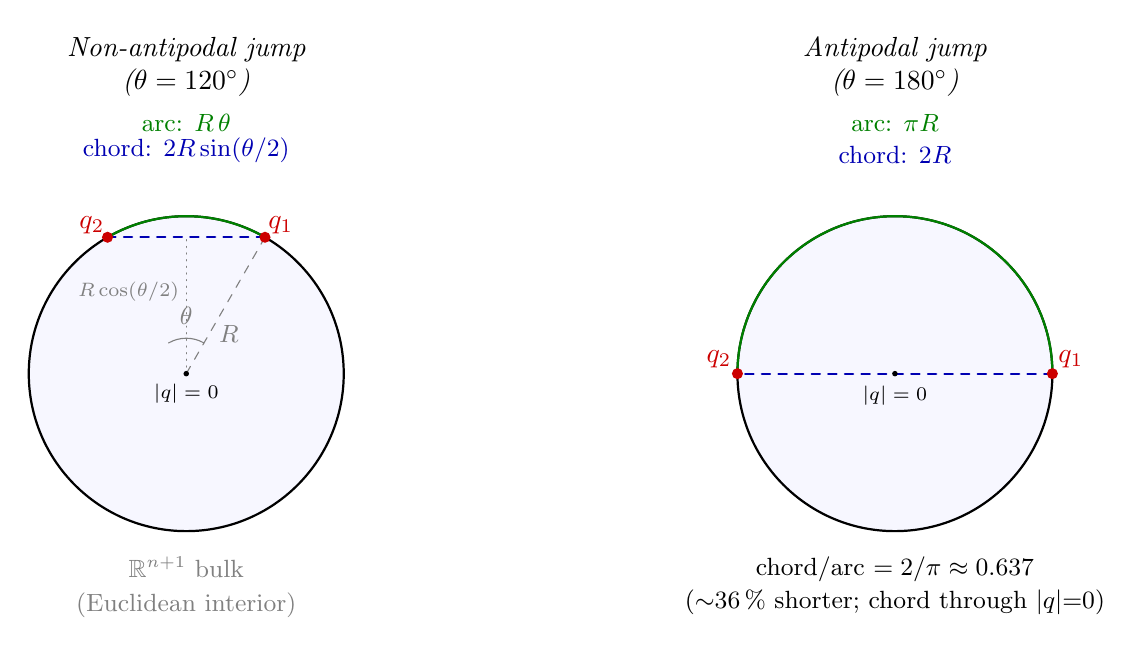
\begin{tikzpicture}[scale=1.0,line cap=round]
  \def\R{2.0}
  % --- Panel A: non-antipodal ---
  \begin{scope}[xshift=-4.5cm]
    \node[align=center] at (0,3.9) {\itshape Non-antipodal jump\\\itshape($\theta = 120^\circ$)};

    % labels above the circle
    \node[green!50!black,anchor=south] at (0,2.95) {\small arc: $R\,\theta$};
    \node[blue!70!black,anchor=south] at (0,2.55) {\small chord: $2R\sin(\theta/2)$};

    \fill[blue!3] (0,0) circle (\R);
    \draw[black,thick] (0,0) circle (\R);

    \coordinate (q1) at (60:\R);
    \coordinate (q2) at (120:\R);

    % chord and arc
    \draw[green!50!black,thick] (q1) arc[start angle=60,end angle=120,radius=\R];
    \draw[blue!70!black,thick,dashed] (q1) -- (q2);

    % radius to q1
    \draw[gray,dashed] (0,0) -- (q1);
    \node[gray,anchor=north west,inner sep=1pt] at ({0.75*cos(60)},{0.75*sin(60)}) {\itshape\small $R$};

    % angle theta marker
    \draw[gray] (60:0.45) arc[start angle=60,end angle=120,radius=0.45];
    \node[gray,anchor=south] at (90:0.5) {\itshape\small $\theta$};

    % apothem
    \draw[gray,dotted] (0,0) -- (0,{\R*cos(30)});
    \node[gray,anchor=east,inner sep=1pt] at (-0.05,{\R*cos(30)*0.6}) {\scriptsize $R\cos(\theta/2)$};

    % origin
    \fill (0,0) circle (1pt);
    \node[anchor=north,inner sep=2pt] at (0,-0.05) {\itshape\scriptsize $\lvert q\rvert = 0$};

    % endpoints
    \fill[red!80!black] (q1) circle (2pt);
    \node[red!80!black,anchor=south west,inner sep=1pt] at (q1) {$q_1$};
    \fill[red!80!black] (q2) circle (2pt);
    \node[red!80!black,anchor=south east,inner sep=1pt] at (q2) {$q_2$};

    \node[gray,anchor=north,align=center] at (0,-2.2) {\small $\mathbb{R}^{n+1}$ bulk\\\small (Euclidean interior)};
  \end{scope}

  % --- Panel B: antipodal ---
  \begin{scope}[xshift=4.5cm]
    \node[align=center] at (0,3.9) {\itshape Antipodal jump\\\itshape($\theta = 180^\circ$)};

    \node[green!50!black,anchor=south] at (0,2.95) {\small arc: $\pi R$};
    \node[blue!70!black,anchor=south] at (0,2.55) {\small chord: $2R$};

    \fill[blue!3] (0,0) circle (\R);
    \draw[black,thick] (0,0) circle (\R);

    \coordinate (p1) at (\R,0);
    \coordinate (p2) at (-\R,0);

    \draw[green!50!black,thick] (p1) arc[start angle=0,end angle=180,radius=\R];
    \draw[blue!70!black,thick,dashed] (p1) -- (p2);

    \fill (0,0) circle (1pt);
    \node[anchor=north,inner sep=2pt] at (0,-0.08) {\itshape\scriptsize $\lvert q\rvert = 0$};

    \fill[red!80!black] (p1) circle (2pt);
    \node[red!80!black,anchor=south west,inner sep=2pt] at (p1) {$q_1$};
    \fill[red!80!black] (p2) circle (2pt);
    \node[red!80!black,anchor=south east,inner sep=2pt] at (p2) {$q_2$};

    \node[anchor=north,align=center] at (0,-2.2) {\small chord$/$arc $= 2/\pi \approx 0.637$\\\small ($\sim$36\,\% shorter; chord through $\lvert q\rvert{=}0$)};
  \end{scope}
\end{tikzpicture}
\caption{Chord through $\mathbb{R}^{n+1}$ versus geodesic arc on $S^n$ (illustrated for $n=1$). The hyperjump trajectory (dashed blue) leaves $S^n$, traverses $\mathbb{R}^{n+1}$, and re-enters at $q_2$.}
\label{fig:chord-vs-arc}
\end{figure}

\begin{table}[H]
\centering
\begin{tabular}{@{}lll@{}}
\toprule
Path & Parameterization & Length \\
\midrule
Geodesic on $S^3$ (normal travel) & $\mathrm{slerp}(X_1, X_2, t)$, with $\lvert X(t)\rvert = \Rgeom$ & $\Rgeom\,\theta$ \\
Chord through $\mathbb{R}^4$ bulk (hyperjump) & $(1-t) X_1 + t X_2$, with $\lvert X(t)\rvert \leq \Rgeom$ & $2\Rgeom\sin(\theta/2)$ \\
\bottomrule
\end{tabular}
\end{table}

Since $\sin(\theta/2)/(\theta/2) \leq 1$ for all $\theta \in (0, \pi]$, the chord is never longer than the arc. The maximum shortcut occurs at the antipodal point ($\theta = \pi$): chord $= 2\Rgeom$ versus arc $= \pi \Rgeom$ --- a reduction of approximately 36\,\%. At bulk speed $u \leq c$ the crossing time is $\Delta\tau = 2\Rgeom\sin(\theta/2)/u$, strictly finite and timelike with respect to the bulk metric.

It must be acknowledged that, from the perspective of an $S^3$-confined observer, the chord traverser arrives sooner than a light signal travelling along $S^3$ between the same endpoints. The effective $S^3$-projected speed for an antipodal chord at bulk speed $c$ is $\pi c / 2 \approx 1.57\,c$. The trajectory is therefore operationally superluminal in $S^3$ projection. This is consistent with the bulk light-cone but in tension with the FTL prohibition in [Nopper 2025a, \S Light-Speed Bound], which is formulated \emph{intrinsically} on $S^3$. The resolution adopted here --- extending the causal-cone definition to the bulk Minkowski metric --- is given as the first-pass closure of subproblem 6 below.

For an antipodal jump the chord passes through $\lvert X\rvert = 0$ at its midpoint; for non-antipodal jumps it passes through a minimum norm $\Rgeom\cos(\theta/2) > 0$. The bulk origin $\lvert X\rvert = 0$ is a point of the auxiliary embedding $\mathbb{R}^4$ at the present cosmic time $\tau$; it is \emph{not} the FLRW initial singularity at $\tau = 0$, although both share the property that the geometric radius vanishes.

\section{A Candidate Dynamical Skeleton: Quaternionic Linear Sigma Model}
\label{sec:sigma}

The SpacetimeTheory designates $\mathbb{R}^4$ as an \emph{auxiliary} embedding space and defines matter only on $S^3$ [Nopper 2025a, \S Foundations]. To make the hyperjump a physical process, the embedding coordinate $X^A$ must be supplemented by independent dynamics: an action principle for fields living on the bulk that admits both $S^3$-localized ground states and chord-like excited trajectories.

We propose, as the simplest candidate skeleton, a Lorentz-invariant linear sigma model with global $O(4)$ symmetry on the bulk $\mathcal{B} = \mathbb{R}_\tau \times \mathbb{R}^4$. The dynamical field is a real 4-component order parameter $\phi^A(X)$ ($A = 1,\dots,4$), not the embedding coordinate $X^A$ itself:
\begin{equation}
\mathcal{L}_\phi = -\frac{1}{2}\, \eta^{MN} \partial_M \phi^A \partial_N \phi^A - \lambda \left( \phi^A \phi^A - v^2 \right)^2
\end{equation}
with $\eta_{MN} = \mathrm{diag}(-c^2, +1, +1, +1, +1)$ and implicit sums over $M,N$ and $A$. Structurally this is the Higgs sector with the field-space vacuum manifold $\{\phi^A\phi^A=v^2\}\cong S^3$. The physical spatial hypersphere remains the geometric locus $\lvert X\rvert=\Rgeom$; identifying that locus with the low-energy brane requires a background profile $\phi_0^A(r)$, where $r=\lvert X\rvert-\Rgeom$, that localizes Standard-Model zero modes near $r=0$.

\textbf{Conventions and dimensions.} Throughout this note we use natural units $\hbar=c=1$ unless otherwise stated. In five spacetime dimensions a canonically normalized real scalar $\phi^A$ has mass dimension $3/2$; the vev $v$ has mass dimension $3/2$; and $\lambda$ has mass dimension $-1$ (confirming non-renormalizability --- see Subproblem 8). The geometric radius $\Rgeom$ has dimension of length and is not the same object as $v$. A complete gravity/localization solution must determine how $v$, $\lambda$, and the background profile $\phi_0^A(r)$ set the brane thickness and the observed geometric radius.

The skeleton does three things:

\begin{table}[H]
\centering
\begin{tabularx}{\linewidth}{@{}lX@{}}
\toprule
Feature & Mechanism \\
\midrule
Brane localization becomes dynamical & Matter confinement is controlled by $\phi_0^A(r)$ rather than imposed as the kinematic constraint $\lvert X\rvert = \Rgeom$ \\
Equations of motion are globally smooth & $\Box \phi^A = 4 \lambda (\lvert\phi\rvert^2 - v^2) \phi^A$ is well-posed everywhere on the bulk, including at $\phi^A = 0$ \\
The central field configuration is non-singular & $V(0) = \lambda v^4$ is finite; leaving the brane encounters a finite barrier, not a divergence \\
\bottomrule
\end{tabularx}
\end{table}

Excitations with energy density above the central barrier $\rho_\star=\lambda v^4$ can in principle push localized states into the bulk along chord trajectories; excitations below the barrier tunnel quantum-mechanically. The appropriate semiclassical estimate is a Euclidean bounce/instanton calculation of Coleman type; once gravity is included, the relevant extension is Coleman--De Luccia rather than a 1D-WKB formula. The parameters $\lambda$ and $v$ control the \emph{brane thickness} $\ell_\perp \sim 1/(\sqrt{\lambda}\,v)$, the \emph{barrier energy density} $\rho_\star=\lambda v^4$, and via $\rho_\star V_{\text{cargo}} c\Delta\tau$ the parametric \emph{energy cost} of transporting an object through the bulk.

This much is a clean dynamical skeleton. It is \textbf{not yet a complete physical theory}.

\section{Open Subproblems}
\label{sec:open}

The skeleton above leaves eight substantial pieces unsupplied. Each is an explicit open problem; the model becomes a candidate physical theory only when all are addressed. Each item is given a textbook-level \emph{first-pass closure} inline --- a starting point, not a final solution. The depth of the residual work varies considerably: items 1--5 reduce to standard exercises in scalar-field cosmology, braneworld gravity, brane localization, gauge symmetry breaking, and dimensional analysis; items 6--7 require dedicated technical follow-ups (causal-structure reformulation, full bounce computation); item 8 is a deferral to a UV-completion programme that lies outside the scope of any single note.

\begin{enumerate}[leftmargin=*]
\item \textbf{Cosmic expansion.} [Nopper 2025a] has $\Rgeom=\Rgeom(\tau)$ (FLRW). The static brane location in the skeleton is incompatible. \emph{First-pass closure:} promote $\Rgeom\to\Phi(\tau)$ with potential $U(\Phi)$ and add a kinetic term $-\tfrac{1}{2}(\partial\Phi)^2$. The homogeneous mode then satisfies $\ddot\Phi+3H\dot\Phi+U'(\Phi)=0$, the standard scalar-field-cosmology equation [Linde 1990]; for slow-roll choices of $U$ this reproduces de Sitter expansion. Full closure requires coupling to 5D gravity (Subproblem 2) so that $H$ and the relation between $\Phi$ and the sigma-model profile are solutions rather than postulates.

\item \textbf{Coupling to gravity.} The bulk is treated as flat. To recover the FLRW geometry as a \emph{solution} rather than a postulate, the action must be coupled to 5D General Relativity,
\begin{equation}
S = \int d^5 X \sqrt{-g} \left[ \frac{\mathcal{R}^{(5)}}{2 \kappa_5^2} + \mathcal{L}_\phi \right],
\end{equation}
in the spirit of Randall--Sundrum-type braneworlds. \emph{First-pass closure:} in the thin-brane limit $\ell_\perp \to 0$, the energy-momentum tensor of the localized $\phi_0^A(r)$ background degenerates to a delta-function shell source near $\lvert X\rvert = \Rgeom$ and the 5D Einstein equations reduce to Israel junction conditions [Israel 1966]; the induced 4D geometry is then standard FLRW with the brane tension $\sigma = \int dr\, V(\phi_0)$ playing the role of an effective cosmological constant. A treatment with finite $\ell_\perp$ requires solving the coupled $(g_{MN}, \phi^A)$ system numerically.

\item \textbf{Standard-Model matter on the brane.} Real matter is not a quaternion sigma model. \emph{First-pass closure:} introduce a 5D Dirac fermion $\Psi$ with a Yukawa mass profile $m_\Psi(r)=h\,f[\phi_0(r)]$ chosen so that $m_\Psi(r)$ changes sign across the brane at $r=\lvert X\rvert-\Rgeom=0$ [Rubakov--Shaposhnikov 1983]. The transverse Dirac equation $\bigl[i\gamma^\perp\partial_r-m_\Psi(r)\bigr]\Psi=0$ then admits a normalizable zero mode with profile $\Psi_0(r)\propto\exp[-\int^r m_\Psi(r')\,dr']$ peaked on $S^3$ and exponentially suppressed in the bulk; this is the 4D Standard-Model fermion. Gauge bosons can be localized by analogous dilaton-type couplings [Dvali--Shifman 1997]. Recovering the full SM spectrum (chirality, generations, Higgs) within this framework is non-trivial but follows established braneworld phenomenology.

\item \textbf{Goldstone-mode mass problem.} The breaking $O(4)\to O(3)$ in field space produces three exactly massless scalars not seen in nature. \emph{First-pass closure:} gauge the connected component $SO(4)$ by introducing gauge fields $A_M^a$ ($a=1,\dots,6$) and replacing the partial derivative by the covariant derivative,
\begin{equation}
\partial_M \phi^A \longrightarrow D_M \phi^A = \partial_M \phi^A - i g A_M^a (T^a)^A{}_B \phi^B,
\end{equation}
plus a Yang--Mills kinetic term $-\tfrac{1}{4} F^a_{MN} F^{a\,MN}$. After symmetry breaking, the three broken generators give three massive vector bosons with masses $m_A\sim gv$; the three Goldstones become their longitudinal components via the Higgs mechanism. The remaining $SO(3)$ gauge bosons stay massless and would need to be either confined or identified with a known sector --- itself a non-trivial phenomenological constraint.

\item \textbf{Determination of $\lambda$ and $v$.} The coupling and vev are unconstrained, so the model is not predictive. \emph{First-pass closure:} in the present setup the transverse direction (radial in the embedding $\mathbb{R}^4$, across the $S^3$ brane) is \emph{non-compact}, so $\ell_\perp\sim1/(\sqrt{\lambda}\,v)$ is a brane-thickness / warping length, not a Kaluza--Klein compactification radius. Sub-millimetre tests of the inverse-square law constrain deviations from 4D Newtonian gravity below roughly $44\,\mu\mathrm{m}$ [Adelberger et al. 2003]; in a non-compact braneworld this translates into a bound on the localization/warping scale, $\ell_\perp\lesssim\ell_{\exp}\approx44\,\mu\mathrm{m}$, and hence $\sqrt{\lambda}\,v\gtrsim1/\ell_{\exp}$. This constrains only the product $\sqrt{\lambda}\,v$; pinning unique values requires an independent observable (e.g.\ a continuum graviton signature in a non-compact transverse direction, a tunnelling rate, a radial-mode mass, or a cosmological constraint on $\Phi$). Note that the precise translation of the laboratory bound into a constraint on $\sqrt{\lambda}\,v$ depends on the unsolved gravity sector (Subproblem 2) and is therefore itself only first-pass.

\item \textbf{Operational FTL versus [Nopper 2025a]'s prohibition.} Chord traversal is timelike in the bulk but superluminal in $S^3$ projection. \emph{First-pass closure:} adopt the bulk Minkowski light-cone of $\eta_{MN}=\mathrm{diag}(-c^2,+1,+1,+1,+1)$ as the \emph{fundamental} causal structure, and reinterpret [Nopper 2025a]'s intrinsic light-speed bound as an emergent statement about $S^3$-confined matter --- strictly valid only for trajectories that remain on the brane. Chord trajectories then satisfy the bulk light-cone. The standard ``FTL implies CTCs by Lorentz-boosting'' argument does \emph{not} directly apply here, because the FLRW embedding picks out a preferred cosmic-time slicing and brane Lorentz boosts are not a true symmetry of the full theory; nevertheless a complete chronology proof must still show that allowed bulk chords cannot be concatenated with brane-confined paths into a closed causal loop. The cost is conceptual: the ``intrinsic'' formulation of light-speed in [Nopper 2025a] must be downgraded to an effective brane-projected bound, and Lorentz invariance of the brane physics becomes approximate rather than exact (constrained by precision tests of vacuum Lorentz invariance --- see Tier 1 below). An alternative --- adding a chronology-protection term that suppresses access to $\phi^A\approx0$ --- preserves the intrinsic formulation but reintroduces an arbitrary suppression scale.

\item \textbf{Tunnelling rate.} A field-theoretic Euclidean bounce calculation of Coleman type [Coleman 1977] should replace the 1D-WKB heuristic; once gravity is included, the appropriate extension is Coleman--De Luccia [Coleman \& De Luccia 1980]. This gives the actual jump amplitude as a function of $\lambda$, $v$, $\phi_0(r)$, and cargo geometry. \emph{First-pass closure:} the relevant process is barrier penetration, not false-vacuum decay --- the system is already in the true vacuum and tunnels through the central bump $V(0)=\lambda v^4$. Dimensional analysis says the bounce action $B$ is controlled by dimensionless combinations built from the wall thickness $\ell_\perp$, the barrier scale $\rho_\star$, the cargo size, and the chord length, so the tunnelling rate per five-volume scales as $\Gamma/\mathcal{V}_5\sim\mu^5 e^{-B/\hbar}$ with $\mu$ a characteristic mass scale. For any parameter set consistent with current non-observation, $B\gg\hbar$ for macroscopic cargo, implying that \emph{unaided} hyperjumps are exponentially suppressed and would require an external coherent source to occur on macroscopic timescales. A full computation of the bounce profile and its prefactor is required to fix the exact exponent.

\item \textbf{UV completion.} The quartic interaction $\lambda(\phi^A\phi^A-v^2)^2$ is non-renormalizable in five spacetime dimensions; the Lagrangian is therefore at best an effective theory below some cutoff $\Lambda$. \emph{First-pass framing:} treat the action as a Wilsonian EFT valid for energies $E\ll\Lambda\lesssim M_{\text{Pl}}^{(5)}$ (the 5D Planck mass after Subproblem 2 is implemented). Within that range the model is predictive in the EFT sense --- operators of dimension $>5$ are suppressed by powers of $E/\Lambda$ --- which suffices for any prediction at sub-Planckian scales, including the chord-traversal energetics. A genuine UV completion (asymptotic safety, embedding in a higher-symmetry or string-theoretic theory) lies beyond the scope of this note and is not supplied here.
\end{enumerate}

A consistent closure of items 1--2 alone would already promote the proposal from a kinematic skeleton to a candidate dynamical theory; items 3--5 and 7 would make it phenomenologically meaningful; item 6 reframes the causal structure of [Nopper 2025a]; item 8 is a deferral to a UV-completion programme.

\section{Experimental Programme}
\label{sec:experiment}

The model's predictions split cleanly into two regimes: properties of the \emph{underlying sigma-model and brane structure}, which are testable with existing or near-term experiments, and properties of \emph{macroscopic chord traversal itself}, which are not testable with any foreseeable technology.

\subsection{Tier 1 --- Tests parasitic on running or near-term experiments}

\begin{table}[H]
\centering
\small
\begin{tabularx}{\linewidth}{@{}p{4.2cm}XX@{}}
\toprule
Observable & What it constrains & Status \\
\midrule
Sub-mm gravity (E\"ot-Wash and successors) & Brane thickness $\ell_\perp$ constrains $\sqrt{\lambda}\,v$ via Subproblem 5 & Currently $\ell_\perp\lesssim 44\,\mu\mathrm{m}$ [Adelberger et al.\ 2003]; next-generation reaches roughly $1\,\mu\mathrm{m}$ \\
Fifth-force / new long-range vector searches & Residual unbroken $SO(3)$ gauge bosons (Subproblem 4) must be confined or below sensitivity & Tight bounds on any massless vector mediator \\
Vacuum Lorentz-invariance / preferred-frame tests & Approximate brane Lorentz invariance required by Subproblem 6 & Existing bounds require any bulk-frame effects to be strongly suppressed \\
CMB scalar/tensor ratio (Planck, LiteBIRD, CMB-S4) & Shape of the inflaton potential $U(\Phi)$ in Subproblem 1 & Tightening $r$ disfavours specific $U(\Phi)$ \\
Spatial-curvature and topology tests (CMB matched circles) & The model presupposes a closed three-sphere universe of finite radius $\Rgeom$ & Data consistent with flat or slightly closed; no positive detection \\
\bottomrule
\end{tabularx}
\end{table}

\subsection{Tier 2 --- Dedicated or next-generation facilities}

\begin{table}[H]
\centering
\begin{tabularx}{\linewidth}{@{}p{5.5cm}X@{}}
\toprule
Observable & What it constrains \\
\midrule
KK-like resonances and missing-energy events at HL-LHC / FCC-hh & Bulk-propagating excitations of $\phi^A$; matter briefly entering the bulk \\
Precision Higgs couplings & Mixing between the SM Higgs and the radial (massive) mode of $\phi^A$ \\
Dark-energy equation of state $w(z)$ & Trajectory of $\Phi(\tau)$ on $U(\Phi)$ \\
\bottomrule
\end{tabularx}
\end{table}

\subsection{Tier 3 --- The hyperjump itself}

Given the exponential suppression in Subproblem 7, no terrestrial experiment can plausibly produce a macroscopic chord traversal. Conceptual milestones, in increasing order of difficulty:

\begin{enumerate}[leftmargin=*]
\item \textbf{Microscopic tunnelling event.} Observation of a single quantum appearing at an unexpected location with a rate consistent with the bounce calculation, after excluding all conventional channels. Astronomically rare for any currently allowed $(\lambda, v, \phi_0)$ background.
\item \textbf{Coherent-source proof of principle.} A configuration raising $\phi^A$ above the central barrier in a small region. The required energy density $\rho_\star = \lambda v^4$ is bounded below indirectly through Subproblem 5's lower bound on $\sqrt{\lambda}\,v$, and for any macroscopic cargo is extreme by any laboratory standard --- qualitatively comparable to the absolute energy-scale problem in warp/wormhole proposals, though here with positive sign.
\item \textbf{Macroscopic chord traversal.} Direct observation of an object appearing near its antipode in less than light-travel time on $S^3$. Not forbidden by the framework, but on no plausible engineering horizon.
\end{enumerate}

\subsection{Falsification criteria}

The proposal is \emph{falsified} (in the strong Popperian sense) if any of the following obtains:

\begin{itemize}[leftmargin=*]
\item Cosmological curvature and topology constraints drive the allowed parameter interval entirely outside the closed three-sphere geometry required by [Nopper 2025a];
\item Sub-mm gravity, fifth-force, and localization constraints leave no overlapping parameter region for $\ell_\perp$, $\lambda$, $v$, and the Standard-Model zero-mode profiles;
\item Precision tests of Lorentz invariance in vacuum exclude the bulk light-cone reformulation of Subproblem 6 at the level required for the chord trajectories to remain consistent with observed brane physics;
\item A graviton spectrum inconsistent with a single non-compact transverse dimension --- for example, a sharp Kaluza--Klein tower with discrete mass spacing characteristic of a \emph{compact} extra dimension, rather than the localized zero mode plus continuum expected for a non-compact transverse direction in the present setup --- is established at any future collider or astrophysical observation.
\end{itemize}

\subsection{Honest summary}

The \emph{theory} is empirically engageable through existing programmes; Tier 1 can strongly constrain it and could potentially falsify specific parameter regions. The \emph{device} --- hyperjump propulsion --- is not on any plausible engineering horizon and would require physics or technology beyond what is currently available.

\subsection{In-principle possibility}

Subject to the obvious disclaimers, the framework contains no in-principle prohibition against constructing a hyperjump device. What it contains are quantitative obstacles: depositing energy density $\rho_\star=\lambda v^4$ coherently in the cargo volume, maintaining quantum coherence of the bulk excitation across the chord, and either accepting the exponentially small spontaneous tunnelling rate or engineering a resonant/stimulated enhancement. Each is severe; none is forbidden by the present skeleton.

In this respect the proposal sits in the same epistemic category as traversable wormholes [Morris \& Thorne 1988] and the Alcubierre warp metric [Alcubierre 1994]: physically permitted within a self-consistent theoretical framework, but with engineering requirements far beyond present extrapolation. One distinguishing structural feature is worth noting: the chord traversal \textbf{does not require violation of the energy conditions of general relativity} --- it requires positive-energy excitations of the sigma-model field above a finite barrier $V(0)=\lambda v^4$, whereas wormhole and Alcubierre constructions require negative energy density (exotic matter). Whether this counts as a \emph{practical} advantage is debatable, since the absolute energy-density scale required here is itself extreme; what is unambiguous is that the \emph{qualitative} obstacle is different.

The honest classification is therefore: \emph{in-principle possible, technologically remote, and structurally distinct from negative-energy-density proposals}.

\section{Note on the Interval-Number Framework}
\label{sec:interval}

Earlier formulations of this proposal invoked the interval-number algebra of [Nopper 2025b] to regularize formal expressions of the type $\rho_{\text{bulk}}\cdot V_{\text{bulk}}\sim \lvert X\rvert^{-3}\cdot \lvert X\rvert^3\to 0\cdot\infty$ that arise if one extends FLRW-style densities into the bulk via the geometric radius $\lvert X\rvert$. Within the sigma-model skeleton above, no such densities appear: the action is governed by the Lagrangian $\mathcal{L}_\phi$, which is finite everywhere. The interval-number framework therefore plays no role in the present formulation. It remains an independent, self-consistent algebraic system [Nopper 2025b] and may still be useful for other extensions of the theory in which genuinely indeterminate forms appear.

\section{Summary}
\label{sec:summary}

\begin{table}[H]
\centering
\begin{tabularx}{\linewidth}{@{}p{5.5cm}X@{}}
\toprule
Framework & Role \\
\midrule
Quaternion-Hypersphere Theory [Nopper 2025a] & Identifies $\mathbb{R}^4$ as the embedding space and supplies the chord-path geometry of the closed $S^3$ universe \\
Quaternionic linear sigma model (this note) & Provides a candidate bulk Lagrangian for an order-parameter field $\phi^A$ whose background profile localizes matter near $S^3$ and whose excited states can enter the bulk \\
\bottomrule
\end{tabularx}
\end{table}

The model is \textbf{geometrically coherent and singularity-free}, but \textbf{not yet dynamically complete}: the eight open subproblems listed above must be closed before it can be considered a candidate physical theory. Each admits a textbook-level first-pass closure sketched inline (with item 8 framed as a Wilsonian-EFT deferral), but full closure of any one item is itself a non-trivial research programme. It introduces, beyond [Nopper 2025a], the $O(4)$-symmetric quartic potential $V(\phi)=\lambda(\phi^A\phi^A-v^2)^2$ with coupling $\lambda$ and vev $v$. These parameters have clean physical interpretations (barrier energy density $\rho_\star=\lambda v^4$, brane thickness $\ell_\perp\sim1/(\sqrt{\lambda}\,v)$, transit-energy cost $\rho_\star V_{\text{cargo}}c\Delta\tau$) but no fixed numerical values at present. The model makes no unique precision predictions yet, and there is no experimental evidence for macroscopic bulk traversal.

\section*{References}
\addcontentsline{toc}{section}{References}

\subsection*{Foundations of this work}
\begin{itemize}[leftmargin=*]
\item {[Nopper 2025a]} Nopper, N. \emph{Quaternion--Hypersphere Theory of Spacetime: A Conceptual Synthesis of Closed FLRW Cosmology, Quaternionic $S^3$ Parameterization, and Relational Time}. 2025. \url{https://github.com/McNopper/SpacetimeTheory/blob/main/SpacetimeTheory.pdf}
\item {[Nopper 2025b]} Nopper, N. \emph{Interval Numbers: A Formal Algebraic Framework for Indeterminate Forms}. 2025. \url{https://github.com/McNopper/ZeroInfinity/blob/main/paper.pdf}
\end{itemize}

\subsection*{Extra dimensions and braneworld models}
\begin{itemize}[leftmargin=*]
\item {[Kaluza 1921]} Kaluza, T. ``Zum Unit\"atsproblem der Physik.'' \emph{Sitzungsberichte der Preu{\ss}ischen Akademie der Wissenschaften} (1921) 966--972.
\item {[Klein 1926]} Klein, O. ``Quantentheorie und f\"unfdimensionale Relativit\"atstheorie.'' \emph{Zeitschrift f\"ur Physik} 37, 895--906 (1926).
\item {[Arkani-Hamed, Dimopoulos \& Dvali 1998]} Arkani-Hamed, N., Dimopoulos, S. \& Dvali, G. ``The hierarchy problem and new dimensions at a millimeter.'' \emph{Physics Letters B} 429, 263--272 (1998).
\item {[Randall \& Sundrum 1999]} Randall, L. \& Sundrum, R. ``A large mass hierarchy from a small extra dimension.'' \emph{Physical Review Letters} 83, 3370--3373 (1999).
\end{itemize}

\subsection*{Speculative spacetime engineering (for comparison)}
\begin{itemize}[leftmargin=*]
\item {[Morris \& Thorne 1988]} Morris, M.~S.\ \& Thorne, K.~S. ``Wormholes in spacetime and their use for interstellar travel: A tool for teaching general relativity.'' \emph{American Journal of Physics} 56, 395--412 (1988).
\item {[Alcubierre 1994]} Alcubierre, M. ``The warp drive: hyper-fast travel within general relativity.'' \emph{Classical and Quantum Gravity} 11, L73--L77 (1994).
\end{itemize}

\subsection*{Sigma models, symmetry breaking, brane localization, tunnelling}
\begin{itemize}[leftmargin=*]
\item {[Linde 1990]} Linde, A. \emph{Particle Physics and Inflationary Cosmology}. Harwood Academic, 1990.
\item {[Coleman 1977]} Coleman, S. ``Fate of the false vacuum: Semiclassical theory.'' \emph{Physical Review D} 15, 2929--2936 (1977).
\item {[Coleman \& De Luccia 1980]} Coleman, S.\ \& De Luccia, F. ``Gravitational effects on and of vacuum decay.'' \emph{Physical Review D} 21, 3305--3315 (1980).
\item {[Israel 1966]} Israel, W. ``Singular hypersurfaces and thin shells in general relativity.'' \emph{Il Nuovo Cimento B} 44, 1--14 (1966).
\item {[Rubakov \& Shaposhnikov 1983]} Rubakov, V.~A.\ \& Shaposhnikov, M.~E. ``Do we live inside a domain wall?'' \emph{Physics Letters B} 125, 136--138 (1983).
\item {[Dvali \& Shifman 1997]} Dvali, G.\ \& Shifman, M. ``Domain walls in strongly coupled theories.'' \emph{Physics Letters B} 396, 64--69 (1997).
\item {[Adelberger et al.\ 2003]} Adelberger, E.~G., Heckel, B.~R.\ \& Nelson, A.~E. ``Tests of the gravitational inverse-square law.'' \emph{Annual Review of Nuclear and Particle Science} 53, 77--121 (2003).
\end{itemize}

\subsection*{Background (Wikipedia)}
\begin{itemize}[leftmargin=*]
\item \href{https://en.wikipedia.org/wiki/N-sphere}{N-sphere}
\item \href{https://en.wikipedia.org/wiki/Quaternion}{Quaternion}
\item \href{https://en.wikipedia.org/wiki/Sigma_model}{Linear sigma model}
\item \href{https://en.wikipedia.org/wiki/Brane_cosmology}{Brane cosmology}
\item \href{https://en.wikipedia.org/wiki/Kaluza\%E2\%80\%93Klein_theory}{Kaluza--Klein theory}
\item \href{https://en.wikipedia.org/wiki/Faster-than-light}{Faster-than-light}
\item \href{https://en.wikipedia.org/wiki/Geodesic}{Geodesic}
\end{itemize}

\subsection*{Inspirational background (science fiction)}

The motivating question of this note --- whether a higher-dimensional shortcut between distant points of our spatial universe could be physically realisable --- is a recurring motif in twentieth-century science fiction. The works listed below served only as \emph{inspiration} for posing the question in the first place; they form no part of the physics or mathematics presented above, and no claim is made that the corresponding fictional devices realise the proposed mechanism.

\begin{itemize}[leftmargin=*]
\item {[Asimov 1951]} Asimov, I. \emph{Foundation}. Gnome Press, 1951. --- hyperspatial jumps.
\item {[Herbert 1965]} Herbert, F. \emph{Dune}. Chilton Books, 1965. --- foldspace navigation.
\item {[Roddenberry 1966]} Roddenberry, G. \emph{Star Trek} (TV series). NBC, 1966. --- warp drive through subspace.
\item {[Lucas 1977]} Lucas, G. \emph{Star Wars: Episode IV -- A New Hope}. 20th Century Fox, 1977. --- hyperspace.
\item {[Banks 1987]} Banks, I.~M. \emph{Consider Phlebas}. Macmillan, 1987. --- discrete jump drives.
\end{itemize}

\end{document}
